\documentclass[12pt, letter]{article}
\usepackage{amsmath, amsfonts,amssymb}
\usepackage{esint}
\usepackage{ragged2e}
\usepackage[a4paper, margin=1in]{geometry}
\usepackage{graphicx}
\usepackage[format=plain, labelfont={bf,it}, textfont=it]{caption}
\usepackage{tikz}
\usepackage{karnaugh-map}
\usepackage[most]{tcolorbox}
\usepackage{fancyhdr}
\usepackage{titlesec}
\usepackage{xcolor}
\usepackage{sectsty}


\definecolor{navyBlue}{RGB}{0, 0, 139}
\sectionfont{\color{navyBlue}\fontsize{30}{30}\selectfont}  
\subsectionfont{\color{navyBlue}\fontsize{18}{18}\selectfont}
\subsubsectionfont{\color{navyBlue}\fontsize{13}{13}\selectfont}
\setlength{\parskip}{\baselineskip}


\usetikzlibrary{matrix,calc}
\graphicspath{{../Images/}}
\setcounter{secnumdepth}{0}
\definecolor{bg}{RGB}{235, 235, 235}

\title{CPU Lab}
\author{Hashim Chaudhry - 3762}
\date{November 2021}

\begin{document}
	\begin{titlepage}
		\maketitle
		\thispagestyle{empty}
	\end{titlepage}
	
	\raggedright
	
	\section{mARMi 16}
	\hrule
	\bigskip
	
	mARMi 16 is a 16 bit minimal ARM-like CPU that is able to execute load, store, conditional, arithmetic, and logical instructions. The following sections are intended to provide documentation on the micro-architecture of the CPU's hardware along with providing example assembly and machine files that can be used to test the CPU's various instructions. The full CPU schematic is shown below.
	\bigskip
	
	\begin{figure}[h]
		\centering
		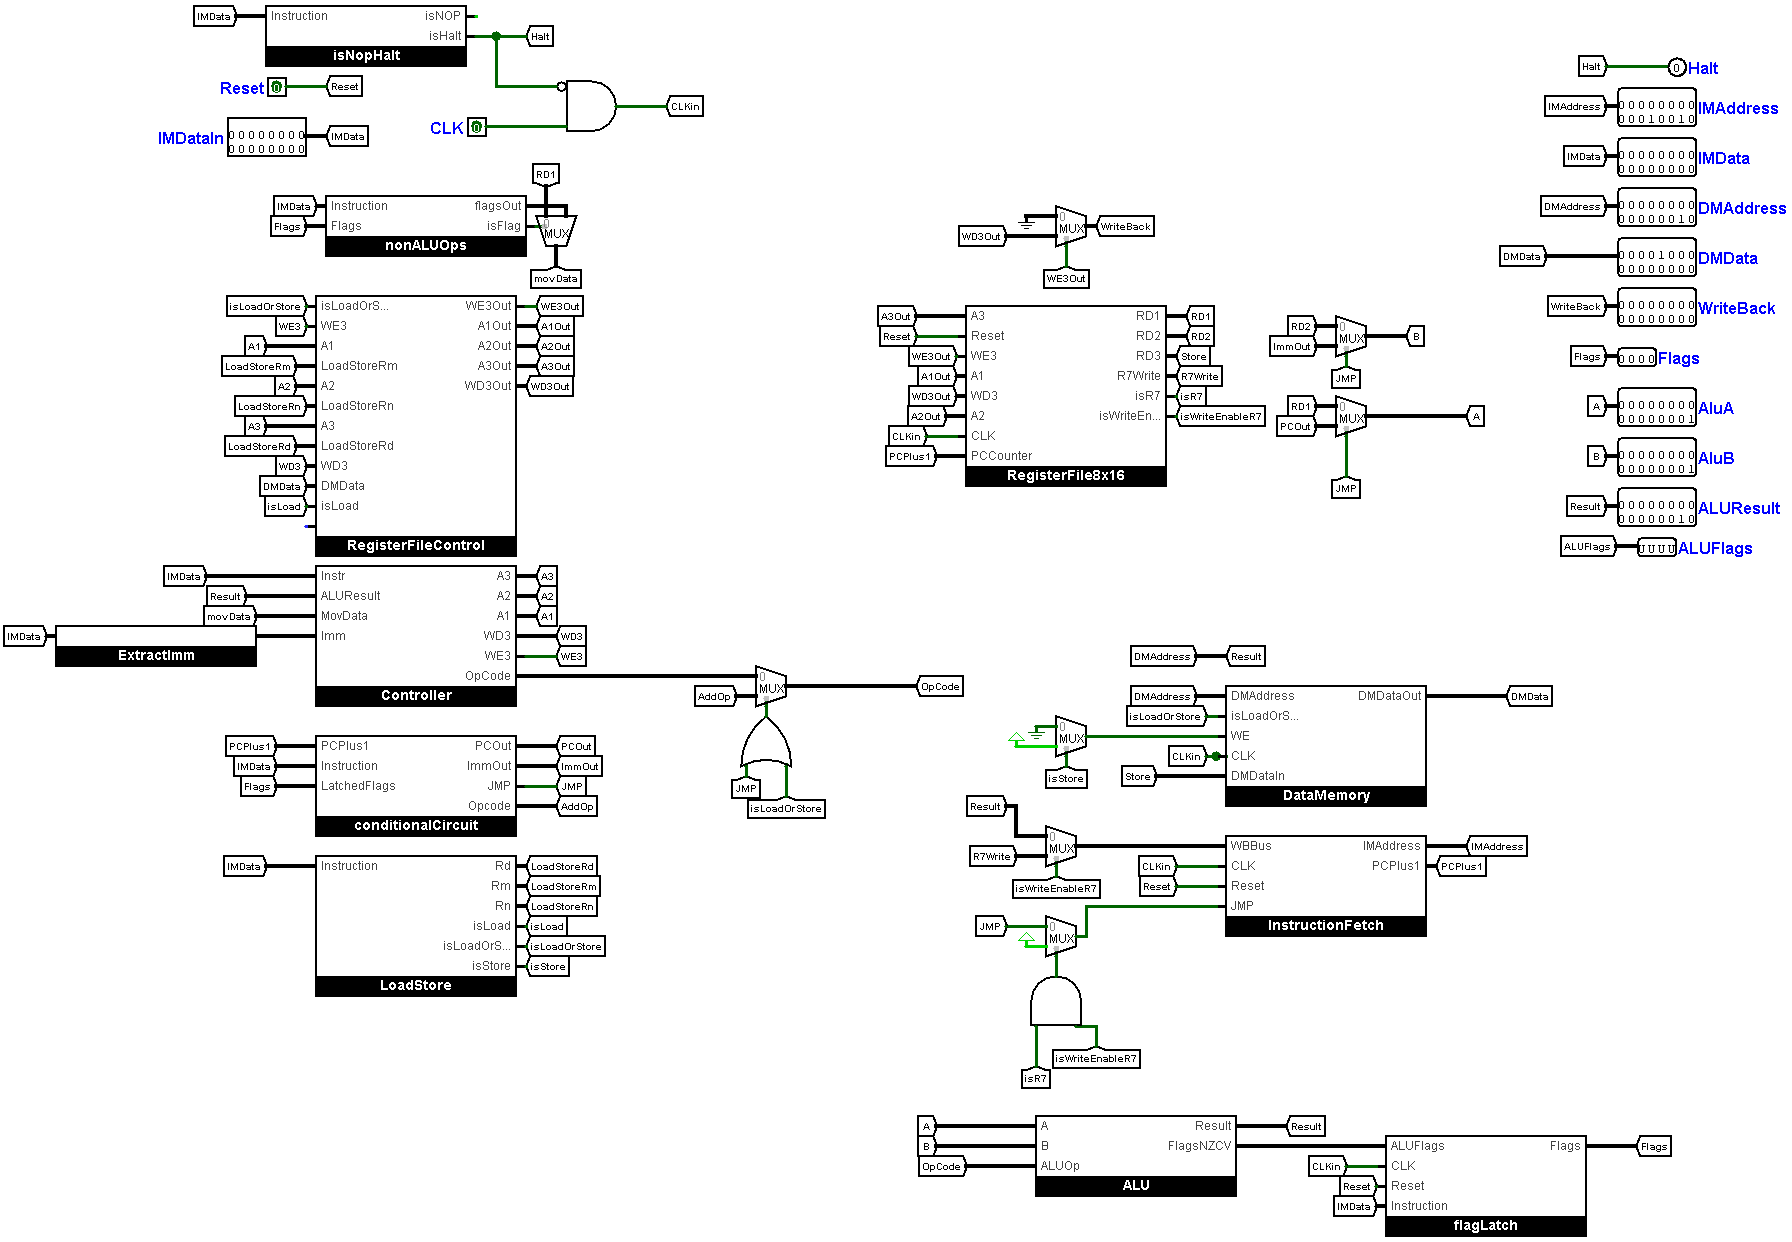
\includegraphics[scale = 0.25]{CPU}
		\caption{mARMi 16 CPU}
		\label{fig:CPU}
	\end{figure}

	mARMi consists of 4 main components: a register file, an instruction fetch unit, a Control Unit, and an ALU. 
	\bigskip

	\hrule
	\newpage
	
	\subsection{Instruction Fetch}
	The instruction fetch unit is designed to fetch the current instruction address being executed from ROM and then store it in a program counter, called $IMAddress$. We also provide a separate output called $PCPlus1$, which provides the address of the next instruction, or $IMAddress + 1$, and is routed to register $R7$ in our register file. 
	
	The instruction fetch takes in 3 inputs: a system wide clock input, a system wide reset input, a $JMP$ flag, and a $WBBus$ input. $WBBus$ supplies an address based on if a branch instruction was executed. The $JMP$ input acts as a flag. If $JMP$ is HIGH, then we allow $WBBus$ to be accepted as the next instruction in our program counter. Otherwise, we use \textit{IMAddress + 1} as the next instruction. 
	
	\begin{figure}[h]
		\centering
		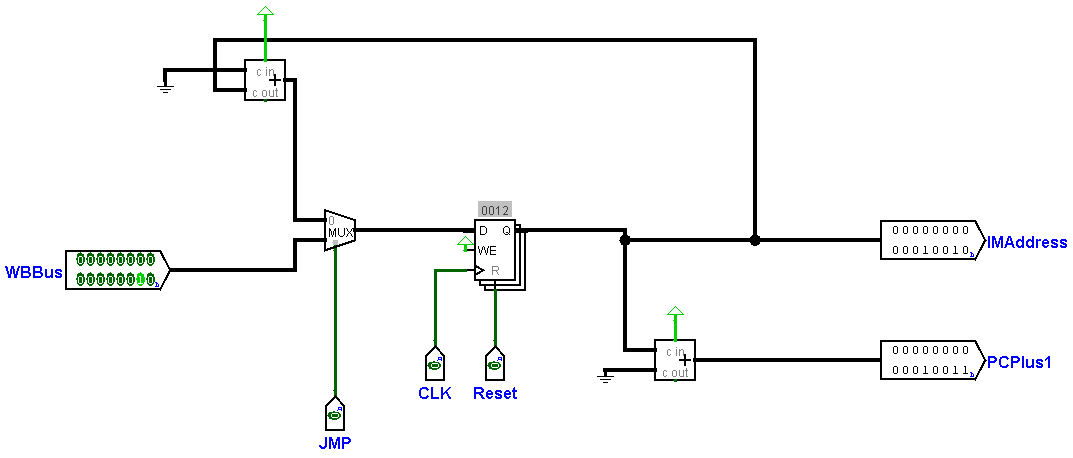
\includegraphics[scale = 0.4]{InstructionFetch}
		\caption{Instruction Fetch Unit}
		\label{fig:InstructionFetch}
	\end{figure}

	The write enable to this register is always high, as it is updated every clock cycle. Computing \textit{IMAddress + 1} is done by adding the current address to 0 and providing a carry-in that is always high. 
	
	\subsection{Arithmetic and Logic Unit}
	
	The arithmetic and logic unit (ALU) is a unit that performs all arithmetic and logical instructions. The ALU selects the correct value to output on \textit{Result} based by using a multiplexer with \textit{ALUOp} as the selector. The \textit{ALUOp} bits are the 4 bits after the first 2 most significant bits on an ALU instruction. All inputs to the ALU are controlled by our control unit and register file. The ALU uses two sub circuits: a FlagController circuit and an ALU shifter circuit. The FlagController circuit computes the carry and overflow flags and the ALU shifter computes the shift output. For shift instructions, the lower 4 bits of input \textit{B} are extracted to tell us the shift amount.
	
	\newpage 
	\begin{figure}[t]
		\centering
		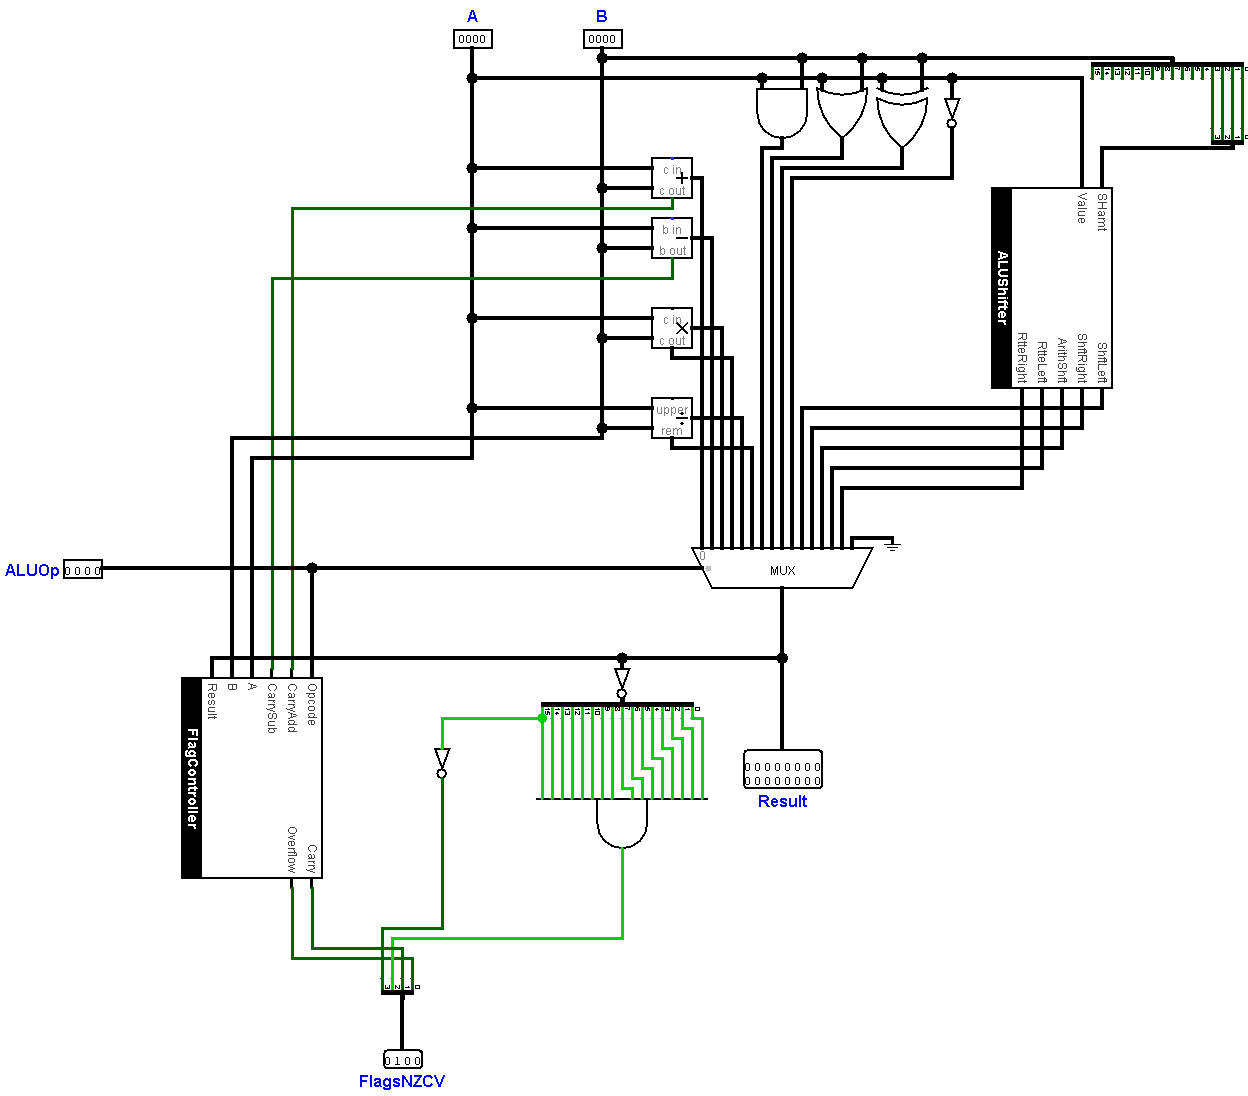
\includegraphics[scale = 0.3]{ALU}
		\caption{Arithmetic and Logic Unit}
		\label{fig:ALU}
	\end{figure}
	
	\subsubsection{ALUShifter}
	
	The ALUShifter circuit below computes the a shift on \textit{A} based on the shift amount \textit{SHAmt}. We then compute each shift output them on their respective lines. These outputs are then routed to the final multiplexer on the ALU. 
	
	\begin{figure}[h]
		\centering
		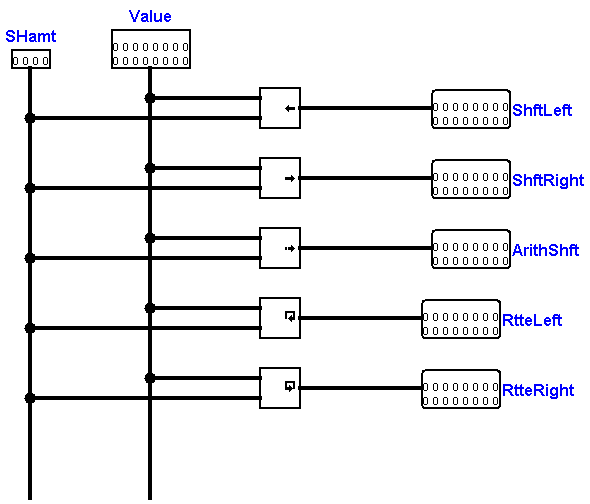
\includegraphics[scale = 0.25]{ALUShifter}
		\caption{Shift Unit for ALU}
		\label{fig:ALUShifter}
	\end{figure}

	\subsubsection{FlagController}
	The FlagController unit uses a more complex circuit to compute carry and overflow flags for addition and subtraction. It takes in the opcode of the CPU to determine whether an ADD or SUB instruction was called, along with \textit{A}, \textit{B}, \textit{Result}, and the carry outs from the adder and subtractor.
	
	\begin{figure}[h]
		\centering
		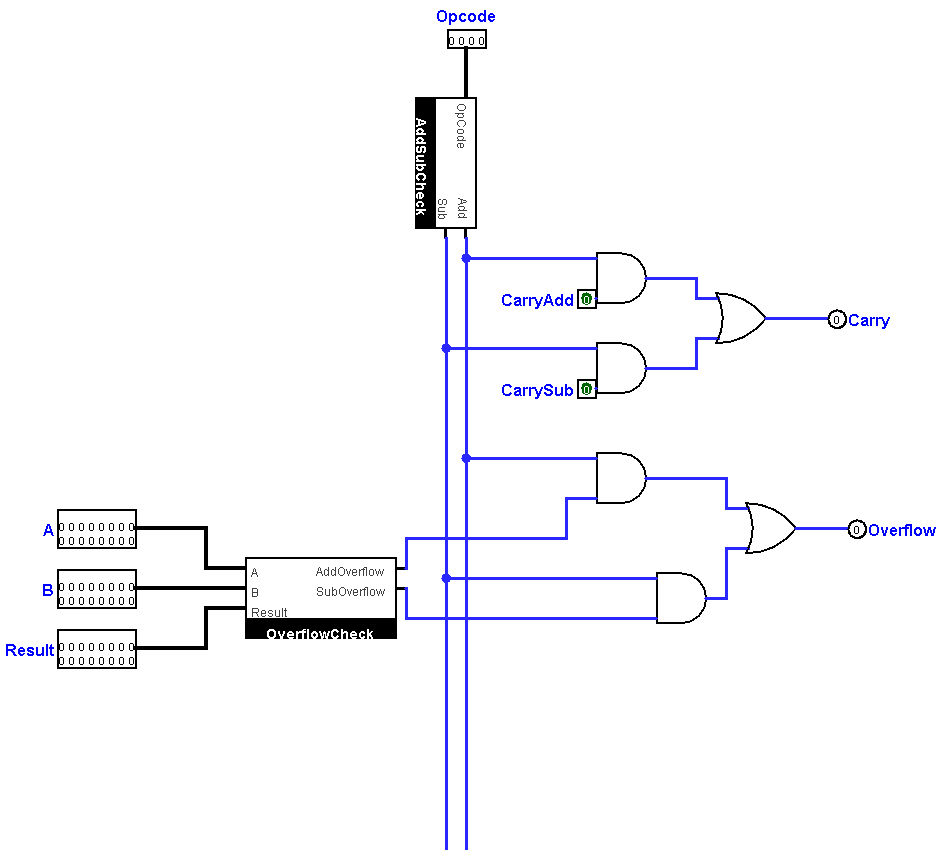
\includegraphics[scale = 0.25]{FlagController}
		\caption{Flag Controller for ALU}
		\label{fig:FlagController}
	\end{figure}

	The AddSubCheck unit allows us to mask the carry and overflow flags on all instructions other than ADD or SUB and also allows us to correctly output carry and overflow based on whether we executed an ADD or SUB instruction. 
	
	\begin{figure}[h]
		\centering
		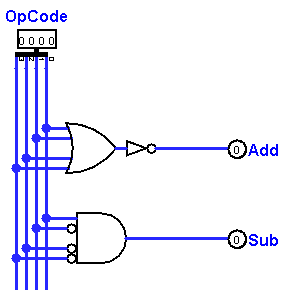
\includegraphics[scale = 0.3]{AddSubCheck}
		\caption{AddSubCheck unit in FlagController}
		\label{fig:AddSubCheck}
	\end{figure}

	The overflow check unit checks an overflow based on the values of \textit{A}, \textit{B}, and \textit{Result}. It has two outputs, an overflow flag for ADD and another for SUB, which are tied to the final overflow flag output for FlagController.An overflow is defined for addition when the sign of the two operands is the same but the result sign is different, and for subtraction it is defined as when the operands have different signs and the result has the same sign as the subtrahend. The sign bit in two's complement is the high bit and, as such, is extracted in OverflowCheck. 
	
	\newpage
	
	\begin{figure}[t]
		\centering
		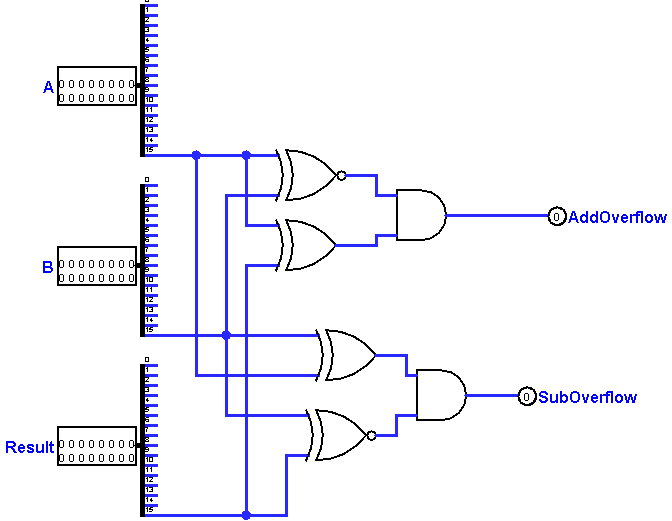
\includegraphics[scale = 0.3]{OverflowCheck}
		\caption{OverflowCheck unit in FlagController}
		\label{fig:OverflowCheck}
	\end{figure}

	The final flags, \textit{Zero} and \textit{Negative}, are computed using gates. The \textit{Zero} flag checks whether each result bit is zero via an AND gate, and the \textit{Negative} flag is set if the high bit of result is set. This is done directly on the ALU. 
	
	\subsection{Latched Flags}
	
	An important part of our ALU is properly supplying arithmetic operation flags so that conditional branches work correctly. However, we only want our flags to be set only when an ALU operation is executed. (Branch instruction don't change the latched flags even though they go through the ALU). As such, a dedicated register keeps track of these flags.
	
	\begin{figure}[h]
		\centering
		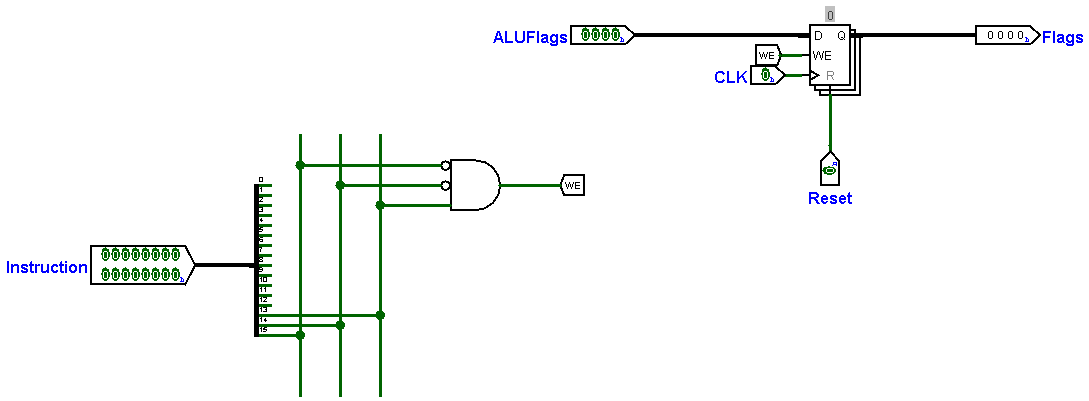
\includegraphics[scale = 0.3]{FlagLatch}
		\caption{FlagLatch unit}
		\label{fig:FlagLatch}
	\end{figure}

	The Flag Latch circuit allows uses the higher 3 bits of the instruction read from memory to determine whether an ALU instruction was encountered. This acts as a write enable for our flag latch register. If it is enabled, the flags from the ALU are saved and are otherwise thrown away. We also provide a system wide reset and clock for this unit. 
	\newpage
	
	\subsection{Register File}
	
	The register file is an 8x16 unit that saves values from the ALU and stores loaded values from memory. It takes 3 three bit address inputs, \textit{A1}, \textit{A2}, and \textit{A3}, where \textit{A3}, is largely intended to be read on \textit{RD3} only for STR instruction and written for writebacks  on \textit{WD3} for other operations. We can write to \textit{A3} based on whether or not \textit{WE3} is HIGH, in which case the value on \textit{WD3} is added to the appropriate register. The coordination of these inputs is largely controlled by the Control Unit, which is discussed later. Demultiplexers are largely used to write to correct registers and multiplexers are used to read from correct registers based on the addresses supplied.
	\bigskip
	
	\begin{figure}[h]
		\centering
		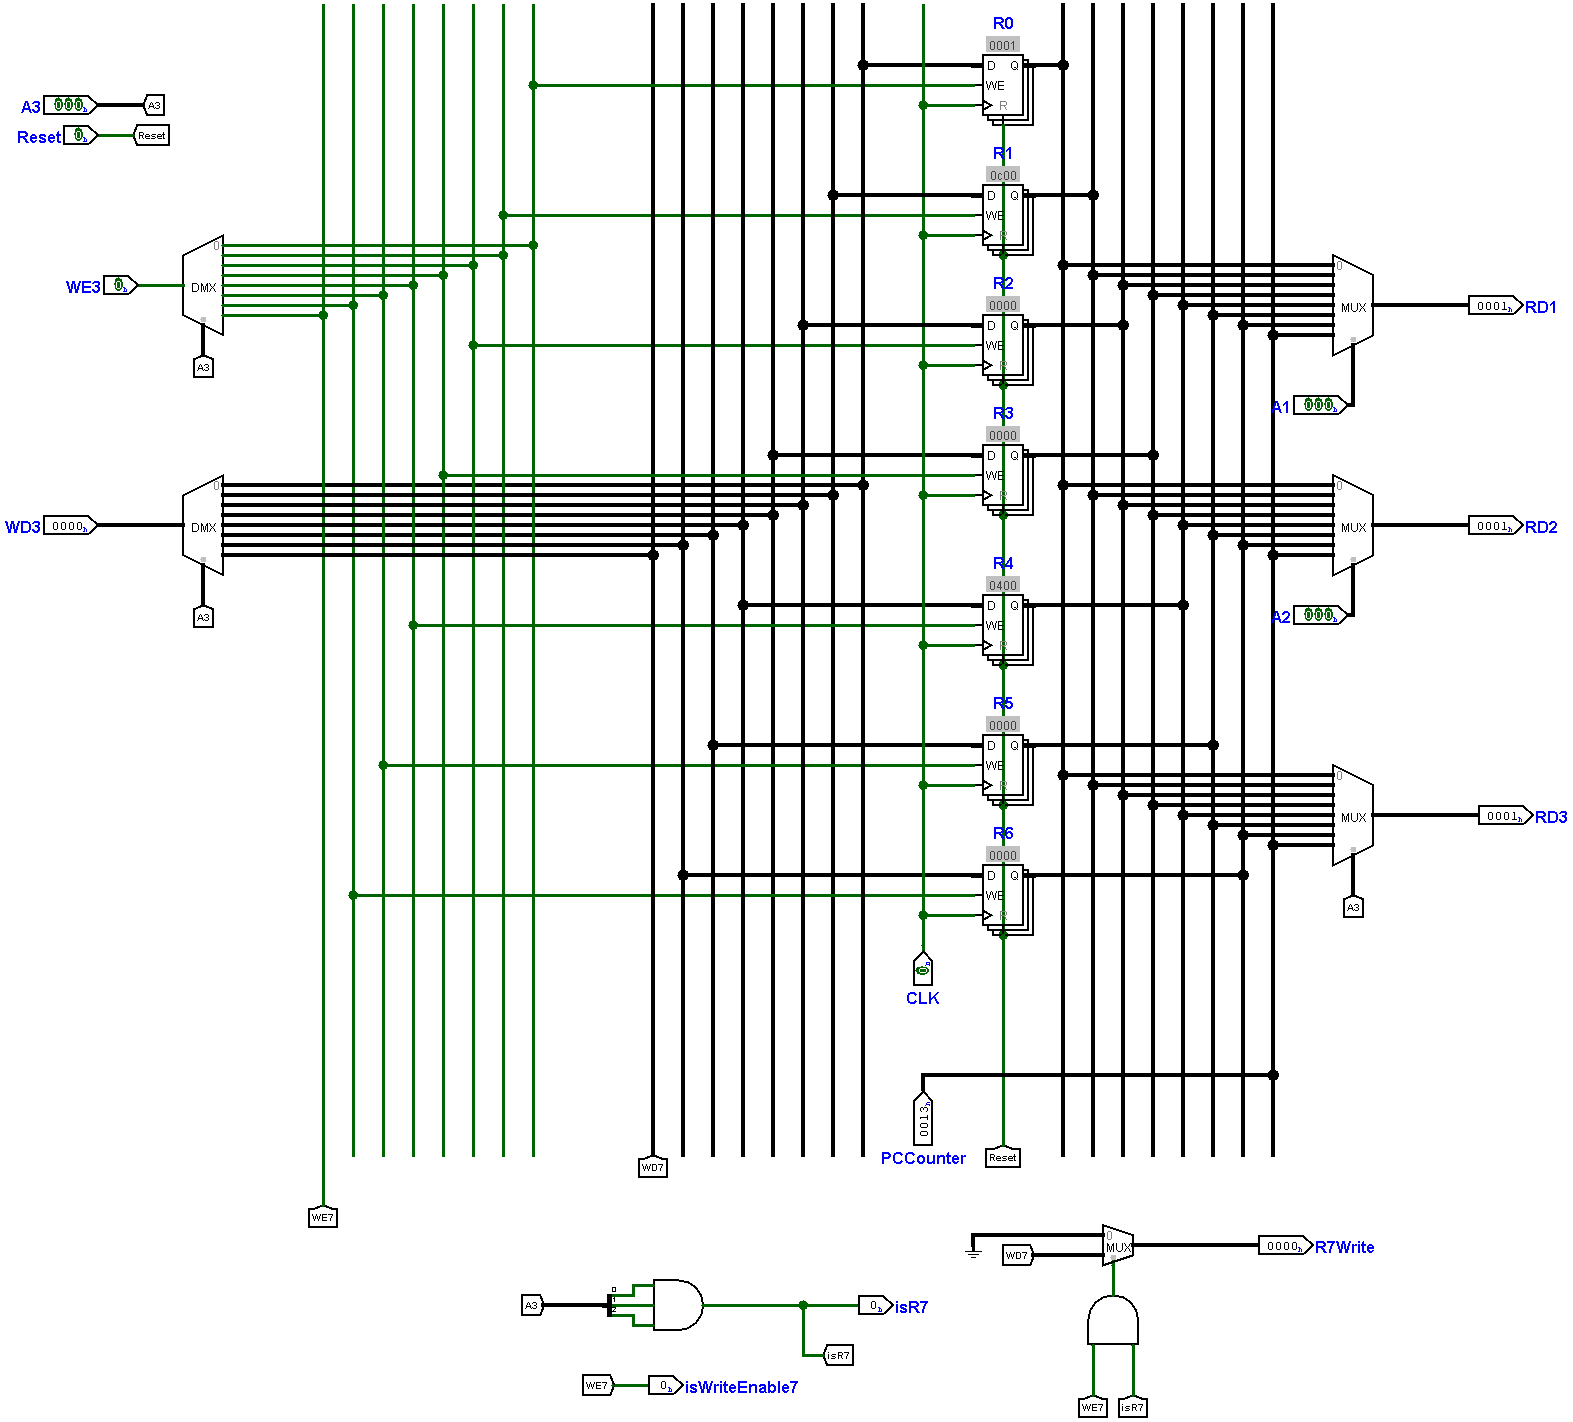
\includegraphics[scale = 0.2]{RegisterFile}
		\caption{Register File for CPU}
		\label{fig:RegisterFile}
	\end{figure}
	
	Register \textit{R7} is a special register that is reserved for the program counter. However, to allow additional functionality to the mARMi CPU, we allow reads and write to the program counter. The \textit{R7Write} output checks to see if the write enable is on and if we are accessing register \textit{R7}, and if so, outputs the data on \textit{R7} write. The output \textit{isR7} is an output flag that lets other outside components, notably the instruction register and writeback paths, in the CPU know that we are writing to the program counter. Reading from \textit{R7} is done by the multiplexers on the output, which will select the correct register based on the read address. 
	
	
	\newpage
	
	\subsection{Data Memory (RAM)}
	
	The data memory module for our CPU acts as 64K RAM for storing values out of registers asynchronously. It accepts a write enable input that allows writes, a \textit{DataIn} value to write, and a \textit{isLoadOrStore} flag that controls a multiplexer and determines whether the address is the result of an LDR or STR instruction. \textit{DMDataOut} simply outputs the data value being asked for based on DMAddress. Note that the output enable is always true in this module, as the Control Unit has a flag that determines whether the output data will be writtin back to the register file from RAM.
	
	\begin{figure}[h]
		\centering
		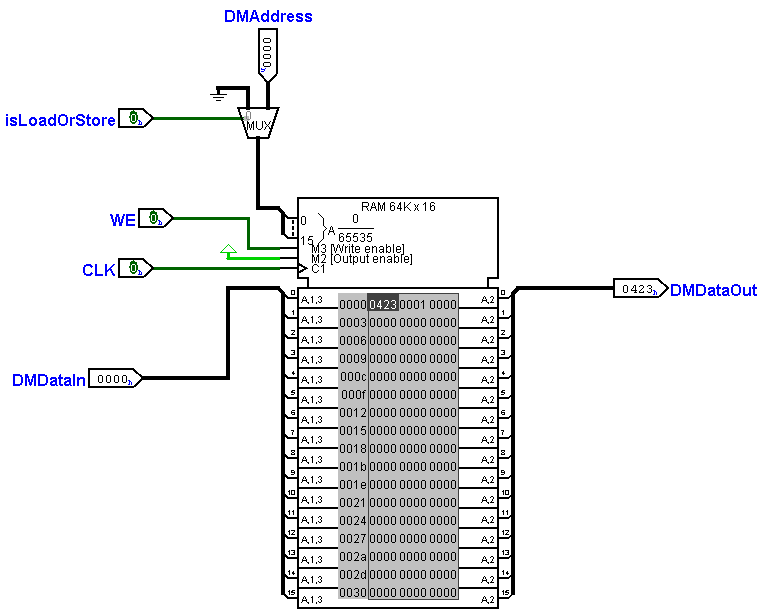
\includegraphics[scale = 0.25]{DataMemory}
		\caption{Data Memory module for CPU}
		\label{fig:DataMemory}
	\end{figure}

	\subsection{NOP and HALT} 
	The isNopHalt module tests for NOP instructions and HALT instructions and outputs a flag on the respective output. The NOP instruction flag is not used in this CPU as the NOP instruction does not activate any units in the CPU. It is, however, provided for convenience should later added modules in the CPU require such a flag. The Halt flag is used to control the CPU's access to the clock.
	
	\begin{figure}[h]
		\centering
		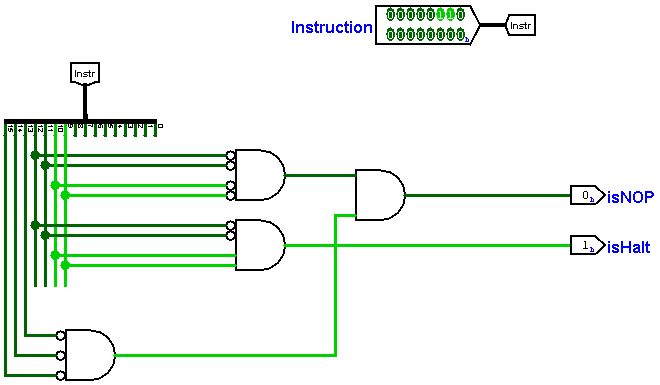
\includegraphics[scale = 0.3]{isNopHalt}
		\caption{Module testing for NOPs and Halts}
		\label{fig:isNopHalt}
	\end{figure}
	\newpage

	\subsection{Control Unit}
	The Control Unit acts as a central brain for decoding instructions and properly setting up other components in the CPU for the instruction. It is a key junction for all instructions and data routing in the mARMi CPU. We consider the $ID$ of an instruction to be the high 4 bits, and the \textit{MSB} to the highest order bit. Our control unit simply extracts needed input values from the instructions and routes them into various subcircuits. Each subcircuit then determines which address that needs to be outputted, along with any signal flags for the CPU.
	
	\begin{figure}[h]
		\centering
		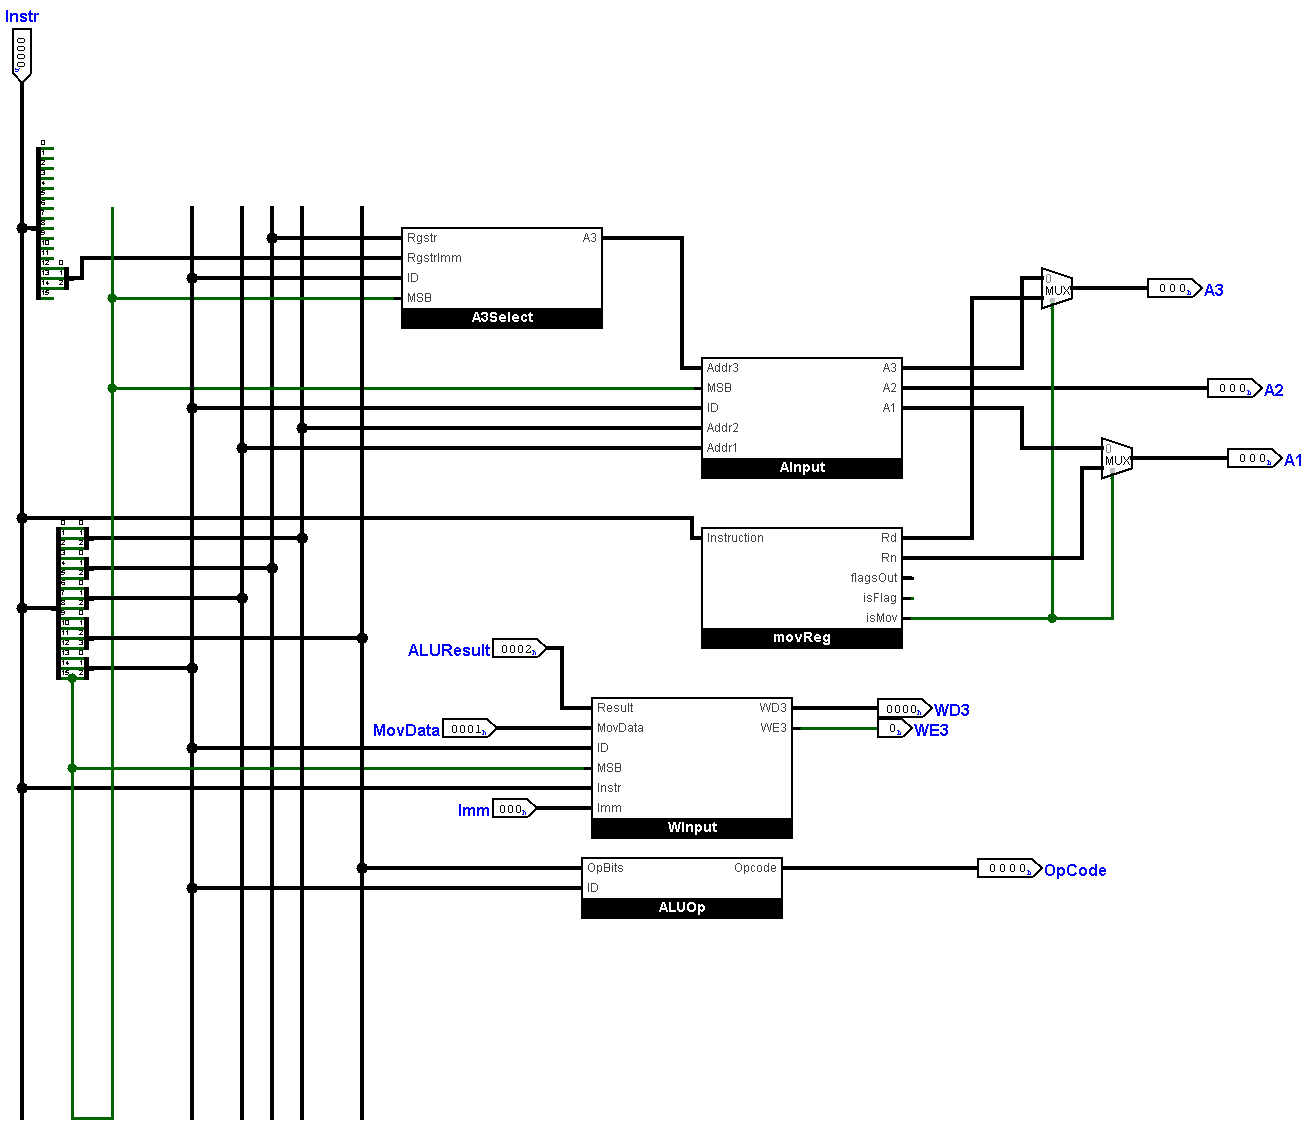
\includegraphics[scale = 0.2]{Controller}
		\caption{Controller}
		\label{fig:Controller}
	\end{figure}

	Each output on the controller corresponds to a value on the register file, except for \textit{OpCode}, which instead outputs an OpCode for the ALU based on whether or not the value an ALU instruction was read. The control units complex circuitry is compartmentalized into various subcircuits.
	
	\subsubsection{A3Select}
	
	The output value for the address on \textit{A3} varies based on the instruction. If the value was a MOV immediate instruction, tested by looking at the MSB, then \textit{A3} outputs the destination register input, called \textit{RgstrImm}. This is extracted in the control unit directly using splitters. Otherwise, if the operation was an ALU operation, we simply output the ALU destination register in the instruction that corresponds to \textit{A3}. This again is also extracted in the Control Unit via splitters.
	\newpage
	
	\begin{figure}[h]
		\centering
		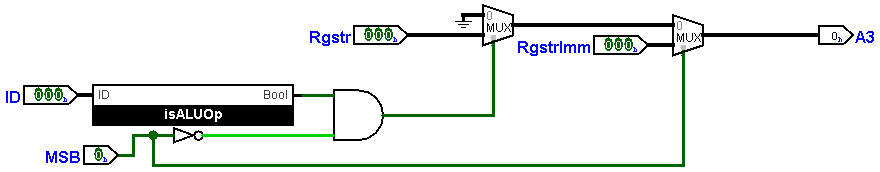
\includegraphics[scale = 0.3]{A3Select}
		\caption{Circuit to correctly extract A3}
		\label{fig:A3Select}
	\end{figure}
	
	\subsubsection{isALUOp}
	This is a subcircuit that tests whether the bits in the instructions constitute an ALU operation, and if so, sets a flag. It is critical for circuits such as the is Latched Flags unit.
	
	\begin{figure}[h]
		\centering
		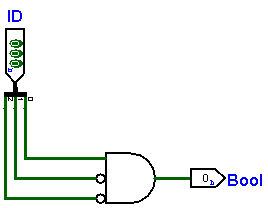
\includegraphics[scale = 0.3]{isALUOp}
		\caption{Circuit that tests whether instruction is an ALU operation}
		\label{fig:A3Select}
	\end{figure}

	\subsubsection{AInput}
	The AInput subcircuit takes in the 3 high order bits and the most significant bit and determines the outputs for \textit{A1, A2,} and \textit{A3} based on the instruction. The outputs of this subcircuit are routed to the controller output for register addresses. The input \textit{A3} for this unit is directly tied to the output of \textit{A3Select}, and it allows for \textit{A3} to pass if the instruction operations signified a MOV immediate or ALU operation. \textit{A1} and \textit{A2} are only outputted for ALU operations. Otherwise, they are masked.
	
	\begin{figure}[h]
		\centering
		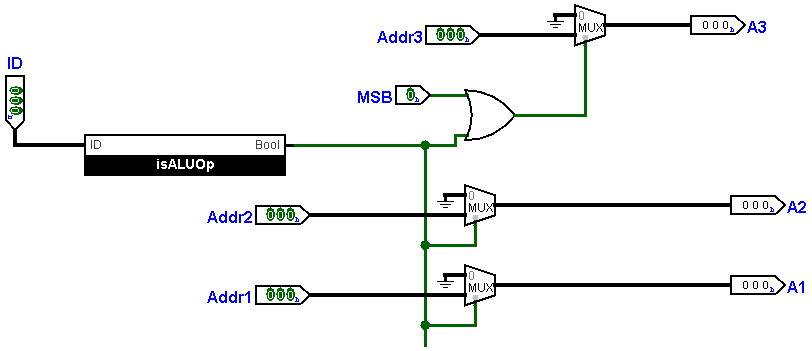
\includegraphics[scale = 0.3]{AInput}
		\caption{Circuit that routes inputs for register addresses}
		\label{fig:AInput}
	\end{figure}

	\subsubsection{movReg}
	The movReg unit tests to see if we are moving data from one register to another, and, if so, outputs the register addresses it has extracted from the instructions as the address lines. It also outputs flags such as \textit{flagsOut}, \textit{isFlag}, and \textit{isMov} to control the multiplexers in the main control circuit and CPU. The \textit{flagsOut} and \textit{isFlag} flags are intneded to notify the controller that we are moving the ALU latched flags into a register. There are two \textit{MOV} instructions, both of which have the same location for \textit{Rd} and so no logic is needed to pick the correct address. However, the value for \textit{Rn} depends on whether we are moving values between registers or moving the ALU latched flags. The multiplexers on the \textit{Rn} output test this condition based on looking directly at the instruction opcode and then use multiplexers to correctly route the data.
	
	\begin{figure}[h]
		\centering
		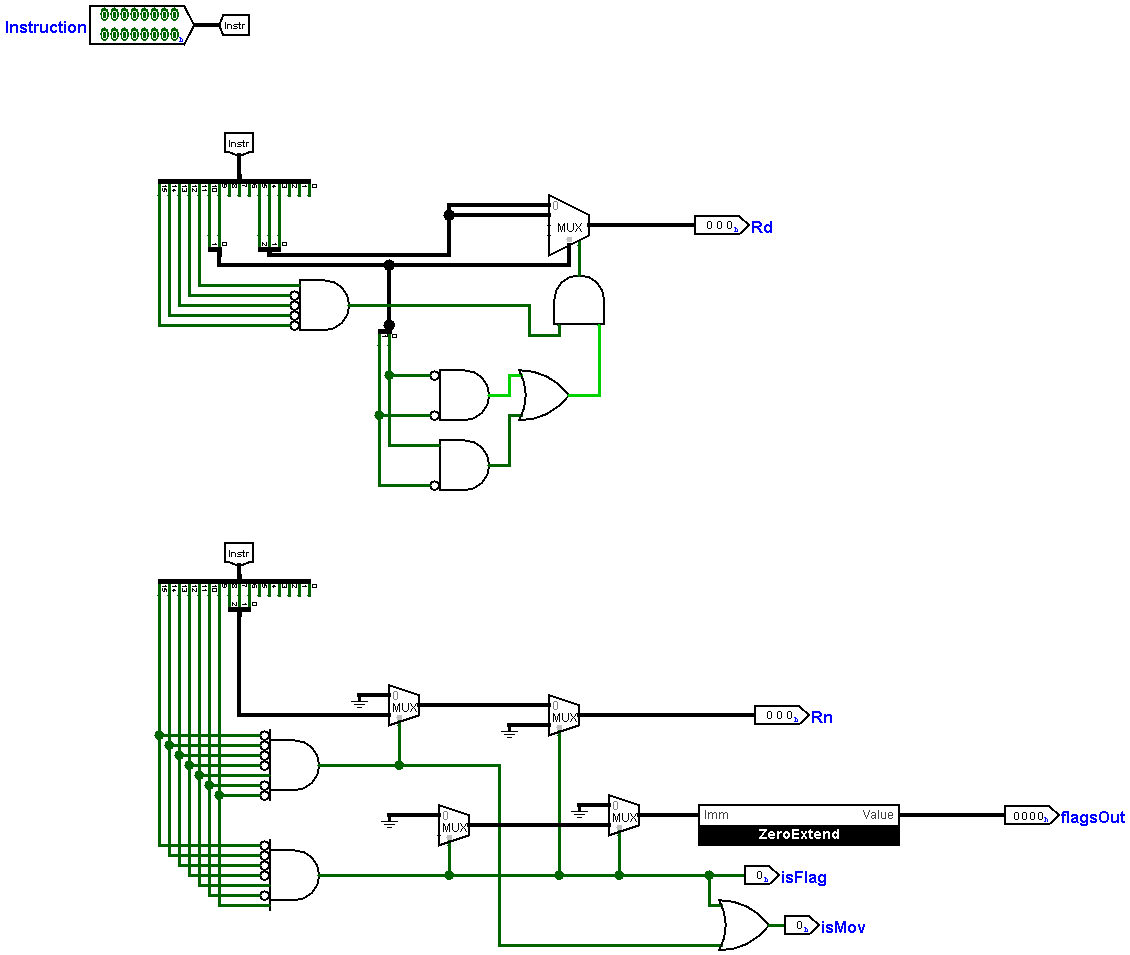
\includegraphics[scale = 0.2]{MovReg}
		\caption{Unit that test to see if instruction is simply moving register values}
		\label{fig:MovReg}
	\end{figure}

	\subsubsection{ZeroExtend}
	The zero extend function takes a 4 bit value and zero extends it. This is intended to be used to sign extend the ALU latched flags when moving ALU flags to a register.
	
	\begin{figure}[h]
		\centering
		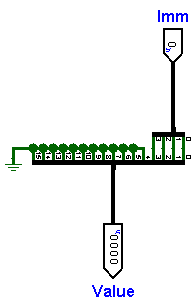
\includegraphics[scale = 0.35]{ZeroExtend}
		\caption{Zero extend circuit}
		\label{fig:ZeroExtend}
	\end{figure}
	
	\subsubsection{WInput}
	This subcircuit determines whether a write enable will turn on and what data should be written if needed. We first test to see if the instruction  is an ALU operation, and if so output the correct write data and enable. We also test for MOV immediate instructions, in which case \textit{WD3} is instead the immediate value of the MOV instruction. Otherwise, if the instruction is a MOV register instruction, we select the MOV data. This is done via multiplexers, where we test the MSB of the instruction for MOV immediate instructions and the \textit{ID} for ALU operations and then select the correct output. In either of these cases, the write enable should be HIGH. We also sign extend our 12 bit immediate value before it is routed. 
	
	\begin{figure}[h]
		\centering
		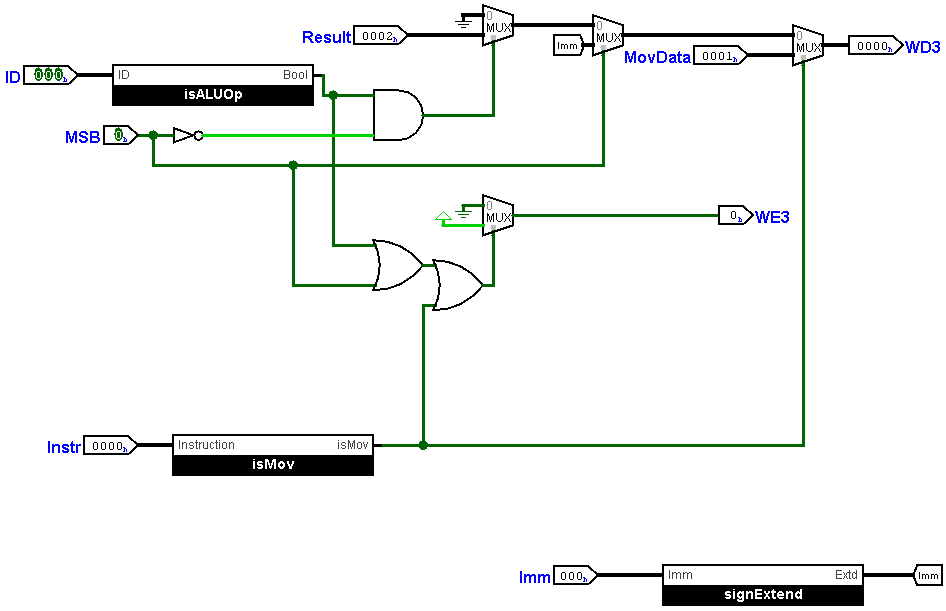
\includegraphics[scale = 0.3]{WInput}
		\caption{Circuit determining write status}
		\label{fig:WInput}
	\end{figure}

	\subsubsection{SignExtend}
	The sign extend subciruit is used to sign extend immediate values before put into a register or used for other operations. It uses a multiplexer based on the high bit to determine whether to extend with 1's or 0's for the high 4 bits.
	
	\begin{figure}[h]
		\centering
		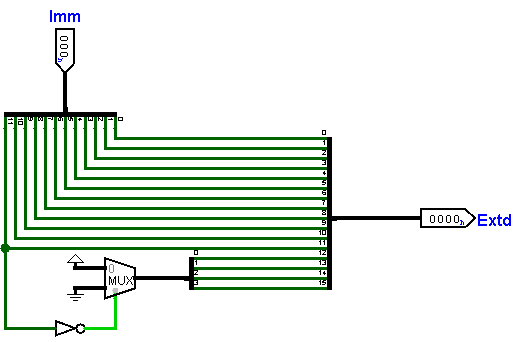
\includegraphics[scale = 0.35]{SignExtend}
		\caption{Sign extend circuit}
		\label{fig:SignExtend}
	\end{figure}

	
	\subsubsection{isMov}
	
	Tests to see whether an instruction intends to move data between two registers. This circuit directly tests the bits necessary to determine whether an operation is a MOV register operation. This unit does not test for MOV immediate instructions.
	
	\begin{figure}[h]
		\centering
		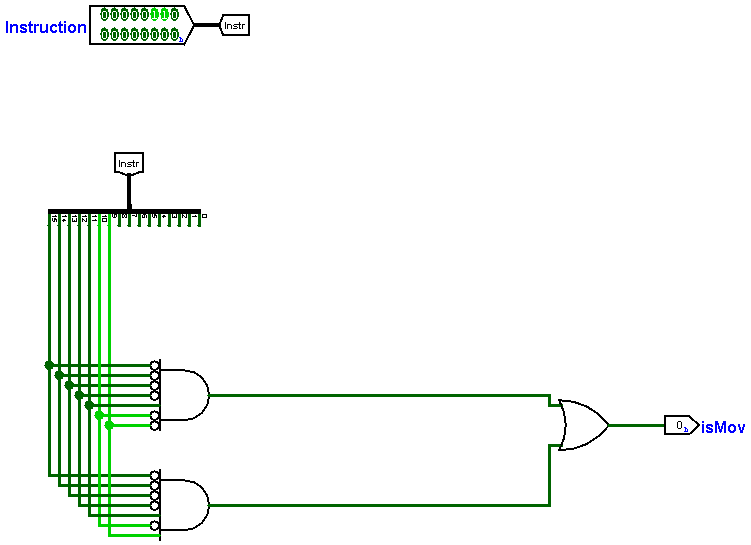
\includegraphics[scale = 0.3]{isMov}
		\caption{Circuit that test for MOV register instruction}
		\label{fig:IsMov}
	\end{figure}
	\newpage
	
	\subsubsection{ALUOp}
	This circuit outputs the ALU operation if our instruction is an ALU operation. In such a case, the multiplexer outputs the ALU operation; otherwise, the output of the ALU is $0000$. We mask the ALUOp outside the controller if the operation does not require the ALU.
	
	\begin{figure}[h]
		\centering
		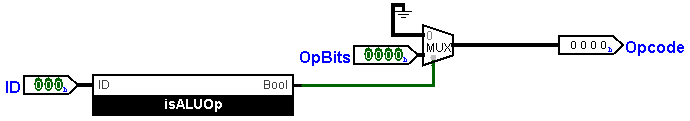
\includegraphics[scale = 0.35]{ALUOp}
		\caption{Circuit that extracts ALU operation if instruction requires ALU}
		\label{fig:ALUOp}
	\end{figure}

	\subsection{LoadStore}
	This circuit is intended to handle memory accesses to and from RAM. It test for the LDR and STR bits, and outputs boolean values on the $isLoad$, $isStore$, and $isLoadOrStore$ flags. It also extracts the necessary register addresses if the instruction is LDR or STR and outputs them using multiplexers. The flag outputs are used on multiplexers in the CPU.  
	\newpage
	 \begin{figure}
	 	\centering
	 	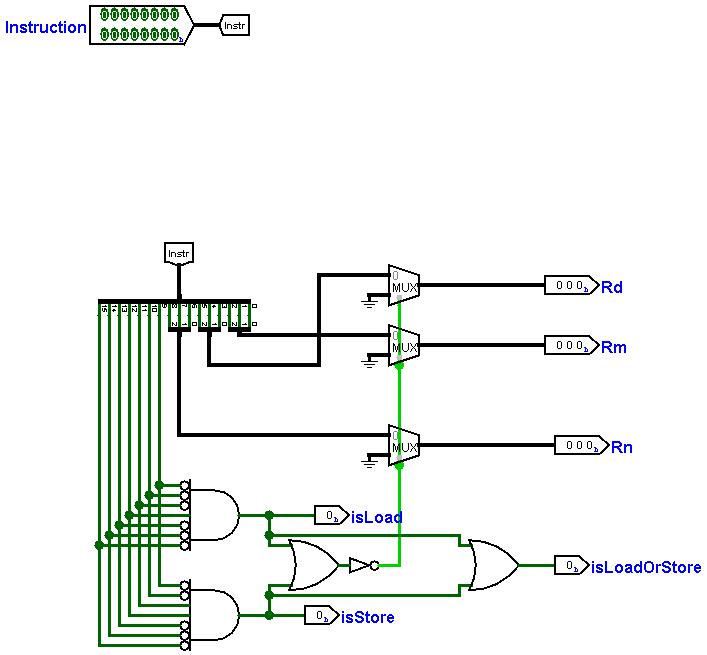
\includegraphics[scale = 0.25]{LoadStore}
	 	\caption{Circuit that sets up LDR and STR instruction registers and Flags}
	 	\label{fig:LoadStore}
	 \end{figure}
 
 	This unit is largely intended to extend some functionality for our Control Unit for more instructions.

 	\subsection{Conditional Circuit}
 	The conditional circuit is intended to be used with instructions that require branching. As such, it takes an input from the latched flags and uses the Z flag to determine whether or not a branch will occur and the immediate value to be passed on based on the result of the conditional implemented with multiplexers. The output of each is then routed to a final 4 input multiplexer which determines what the immediate value will be  based on whether we read in a B, BEQ, or BNEQ instruction, and the condition is met. The select is done directly with the two bits after the two high order bits in the instruction, tell us which branch is needed. We also use an enable which disables this final multiplexer if the instruction is not a branch instruction to mask the output. This immediate value is sign extended before it is finally used. We also provide an ADD opcode output for convenience when this circuit is used elsewhere, as branch instructions will ADD a number to the program counter.
 	
 	  \begin{figure}[h]
 	  	\centering
 	  	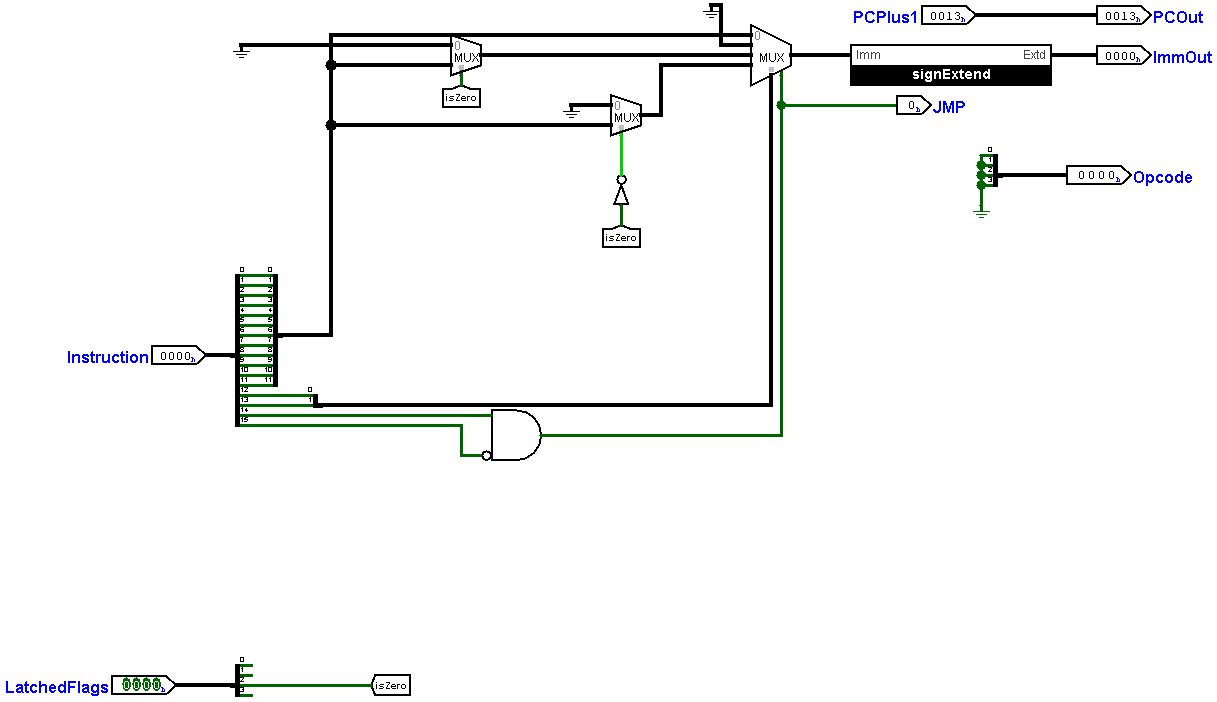
\includegraphics[scale = 0.25]{ConditionalCircuit}
 	  	\caption{Testing and evaluating branch instructions circuit}
 	  	\label{fig:ConditionalCircuit}
 	  \end{figure}
   
   \subsection{Handling Flag Movement}
   
   This circuit handles any non-ALU based operations, notably handling the movement of the latched flags to another register and setting the appropriate boolean flag if necessary. Its primary purpose is to supply the latched flags to a register. Based on the instruction, the output will either output the latched flags, zero extended, or not output anything. 
   
   \begin{figure}[h]
   	\centering
   	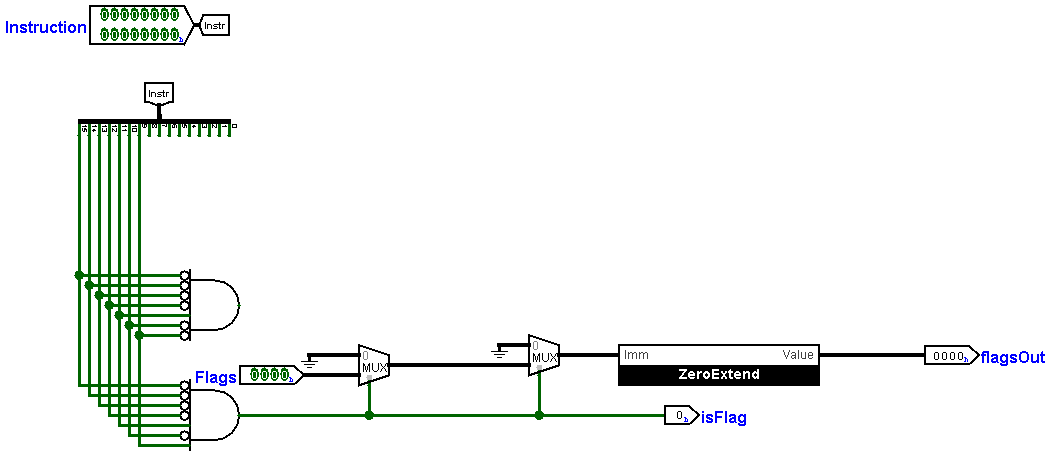
\includegraphics[scale = 0.35]{NonALUOps}
   	\caption{Subcircuit testing non-ALU instructions, notable flag movement instructions}
   	\label{fig:NonALUOps}
   \end{figure}
	
	\subsection{Register File Control}
	The Register File Control is a final check before the necessary data enters the register file, ALU, and other circuits. It is an extension of the Control circuit that largely tests for LDR and STR operations and preps data accordingly. It uses one final stage of multiplexers, with the select on each multiplexer based on the \textit{isLoad} and \textit{isStore} flags, before the data is routed to where it needs to go. Keeping this unit seperate from the control unit allows for easier data routing as multiplexers are all combined into one subcircuit.
	\newpage
	\begin{figure}[h]
		\centering
		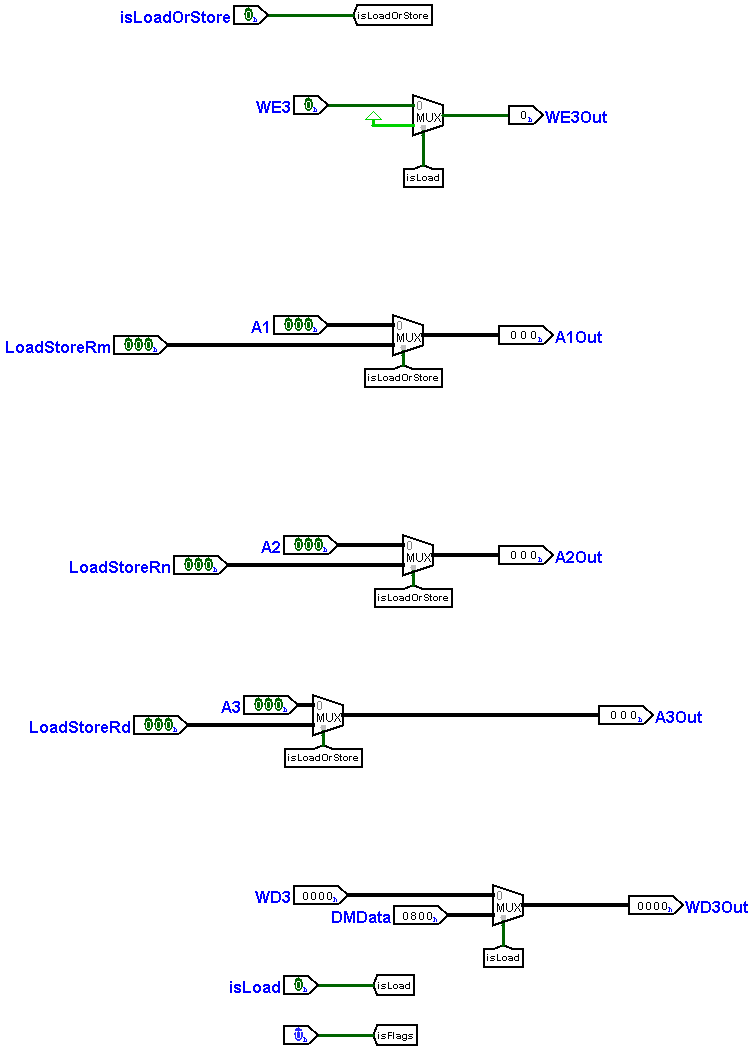
\includegraphics[scale = 0.3]{RegisterFileControl}
		\caption{The Register File Control}
		\label{fig:RegisterFileControl}
	\end{figure} 
	\newpage
	
	\section{Data Routing}
	\hrule
	
	With all necessary components, we can now focus on routing data. All data routing was done with 2 input multiplexers with selects based on the various boolean flags the above modules provided to allow for simple and easy routing. 
	
	The first routing occurs directly out of the control unit for the ALU opcode. If an LDR, STR, or JMP instruction occurred our opcode should be 0000 (ADD). Otherwise, we simply use the opcode the Controller extracted from the instruction. No matter what, our ALU will always compute a result (needed or not),and whether this result is used is determined by various signal flags.
	
	We also need to route between inputs \textit{A} and \textit{B} of the ALU. If the instruction read was LDR or STR, then we know that the \textit{A} should be the program counter and \textit{B} should be the immediate value extracted from the branch instruction that is outputted from the Conditional circuit. Otherwise, if there was not LDR or STR instruction, we simply use \textit{RD1} and \textit{RD2}. As outputted from the main Control Unit. 
	
	We also use multiplexers to route where the result of the ALU goes. This is done with the \textit{isLoadOrStore} flags for the Data memory, \textit{isWriteEnableR7} and \textit{JMP} flags for the instruction fetch unit, and the \textit{WE3} flag for the register file. If none of these flags are ON, then the value is thrown away. For all instructions, data is waiting to be written, but these flags acts as enables that determine whether a write occurs or not. 
	
	We also use a multiplexer for our writeback. If WE3 is on, that means a writeback occurred in the register file, and as such is outputted to the write back display on the front panel controller. Otherwise, zero is displayed. 
	
	The instruction fetch unit also takes in another multiplexer to decide whether a write to R7 occurred or a branch occurred based on the value of the R7 boolean flags that were outputted from the register file. If either of these occurred, the \textit{JMP} flag in the instruction fetch unit is turned ON.
	
	Another data routing occurs based on the MOV register instruction. The Control circuit requires that, for a MOV immediate instruction be supplied as one of its inputs. We use a multiplexer to determine whether \textit{R1}, the source register, is used in the instruction, or the latched ALU flags are the source register, with the flag \textit{isFlag} from the NonALUOp unit determining which one is selected. Again, the Control circuit may throw this value away if the instruction is not a MOV reg instruction (this is done by the isMov unit within the control unit).
	
	Our final data routing process occurs in Data Memory. A multiplexer is used based on whether or not a STR operation occurred. If it does, the write enable for the Data Memory is enabled, and writing is allowed. Otherwise, writing is disabled to the module.
	
	This completes all data routing for the CPU. Our final CPU circuit is shown below, rotate 90 degrees for larger details

	\begin{figure}
		\centering
		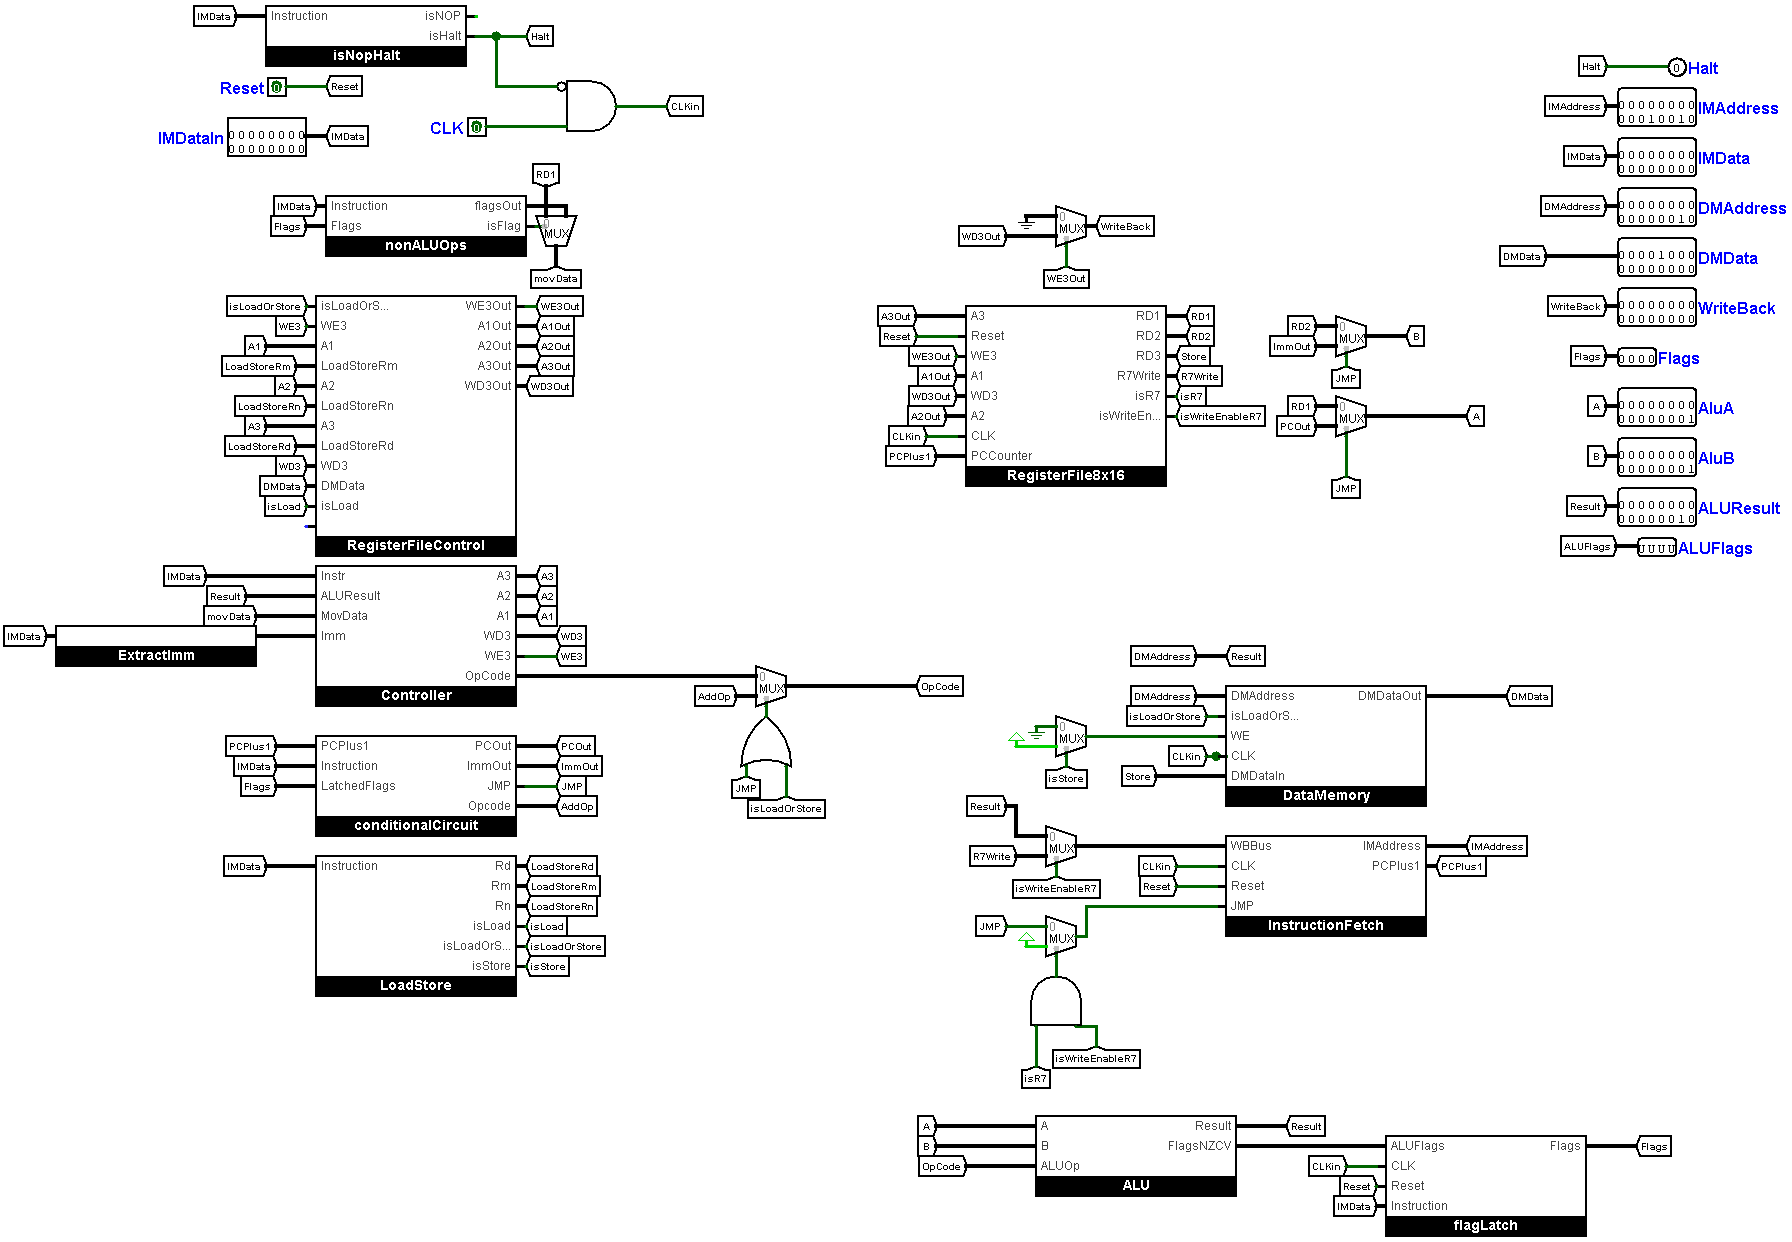
\includegraphics[scale = 0.38, angle = -90, origin =c]{CPU}
		\caption{CPU (rotated)}
		\label{fig:rotateCPU}
	\end{figure}

	
	\section{Test Programs}
	\hrule
	The next few sections provide test circuits that were used on the CPU. There are 4 circuits, each of which test various sets of instructions and expects particular outputs. While each one has a primary aim, the objective is to try to ensure that we get a good mix of instructions such that we test various combinations of instructions on the CPU
	
	\subsection{Testing the "Odd" Movement between Registers} 
	
	The following tests movement between registers, mostly with latched flags and the program counter which are "odd" moves. It also triggers a flag and then supplies a NOP to ensure nothing happens. This program is intended to be seen step by step.
	
		\begin{figure}[h]
			\centering
			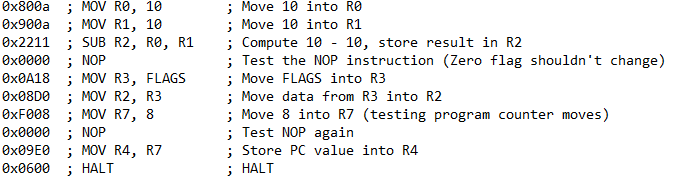
\includegraphics[scale = 1]{movTest}
			\caption{Testing the MOV instructions}
			\label{fig:moveTest}
		\end{figure}
		The assembly for using this in our CPU is below.\\
		\bigskip
		\begin{tcolorbox}[colback = bg, boxrule = 0pt]
			v2.0 raw\\
			v2.0 raw\\
			800a 
			900a
			2211
			0000
			0A18
			08D0
			F008
			0000\\
			09E0
			0600
		\end{tcolorbox}
	
	\subsection{Testing Various ALU operations}
	The following program tests basic ALU operations
	\newpage
	\begin{figure}[h]
		\centering
		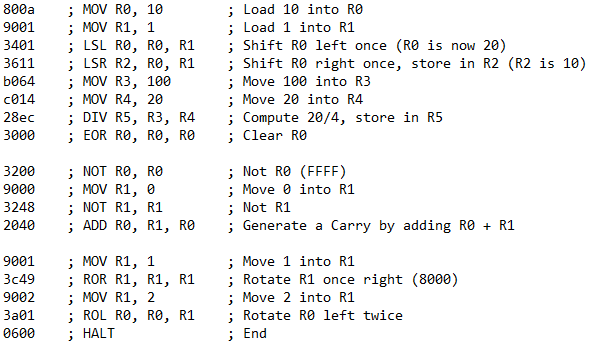
\includegraphics[scale = 1]{aluTest}
		\caption{Testing the ALU}
		\label{fig:aluTest}
	\end{figure}

	The machine code is below
	\begin{tcolorbox}[colback = bg, boxrule = 0pt]
		v2.0 raw\\
		800a 9001 3401 3611 b064 c014 28ec 3000 \\
		3200 9000 3248 2040 9001 3c49 9002 3a01 \\
		0600
	\end{tcolorbox}

	\subsection{Testing Branches}
	The following section intends to test branches. If the code loops infinitely, something is wrong within the CPU. 
	
	\begin{figure}[h]
		\centering
		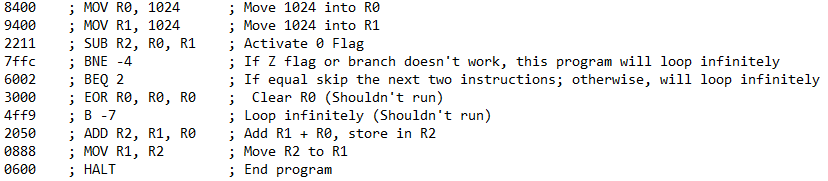
\includegraphics[scale = 1]{branchTest}
		\caption{Testing branch and conditional instruction}
		\label{fig:aluTest}
	\end{figure}

	\bigskip
	
	The machine code is listed below
	\bigskip
	\begin{tcolorbox}[colback = bg, boxrule = 0pt]
		v2.0 raw\\
		8400 9400 2211 7ffc 6002 3000 4ff9 2050\\
		0888 0600\\
	\end{tcolorbox}
	
	\subsection{Load and Store}
	This is the final test program, and it tests load and store operations. It also does branching, as the previous one, along with some ALU operations. Ideally, $0800$ should be at address 0000 and $0C00$ should be at address 0001.
	
	\begin{figure}[h]
		\centering
		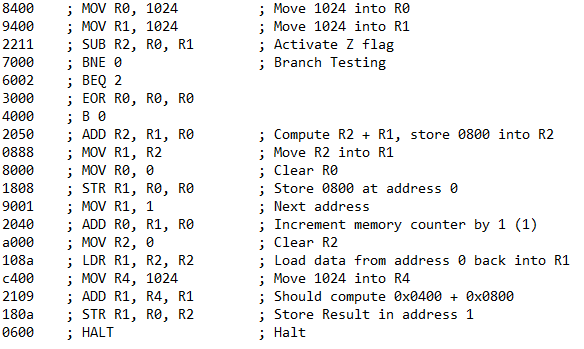
\includegraphics[scale = 1]{loadTest}
		\caption{Testing Load instructions}
		\label{fig:aluTest}
	\end{figure}

	\bigskip
	
	The machine code is listed below
	\begin{tcolorbox}[colback = bg, boxrule = 0pt]
		v2.0 raw \\
		8400 9400 2211 7000 6002 3000 4000 2050 \\
		0888 8000 1808 9001 2040 a000 108a c400 \\
		2109 180a 0600
	\end{tcolorbox}
	
	\bigskip
	
	\subsection{Fibonacci}
	We also provide a Fibonacci assembly program. We list the code as an LST file. To run the program, simply put the Fibonacci number you want to compute in memory at address 0x80.  
	
	\begin{figure}
		\centering
		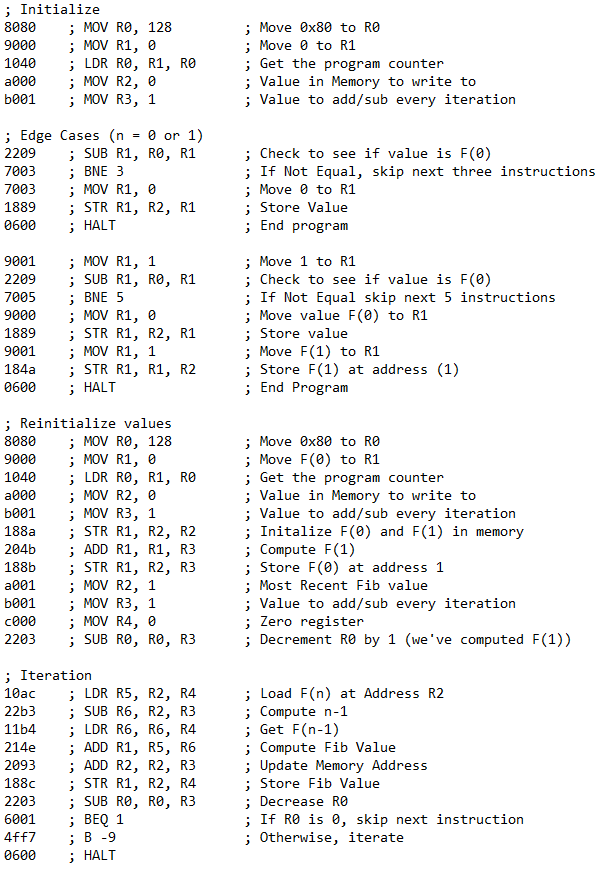
\includegraphics[scale = 1]{fib}
		\caption{Fibonacci Program}
		\label{fig:fib}
	\end{figure}
	\newpage
	The assembly file alone is shown below\\
	\bigskip
	\begin{tcolorbox}[colback = bg, boxrule = 0pt]
		v2.0 raw\\
		8080 9000 1040 a000 b001 2209 7003 9000\\
		1889 0600 9001 2209 7005 9000 1889 9001\\
		184a 0600 8080 9000 1040 a000 b001 188a\\
		204b 188b a001 b001 c000 2203 10ac 22b3\\
		11b4 214e 2093 188c 2203 6001 4ff7 0600\\
	\end{tcolorbox}
	
	\subsection{Testing Register 7 (Program Counter) Operations}
	The following is intended to give a more detailed test of operations on register 7, as it is crucial to the execution of a program and operating errors on it can cause serious problems.
	\begin{figure}[h]
		\centering
		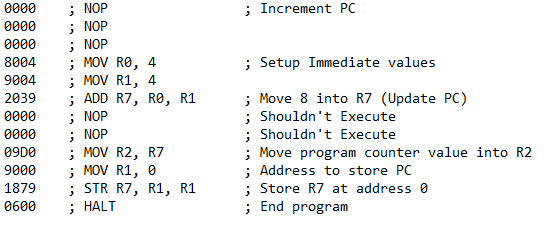
\includegraphics[scale = 1]{pcTest}
		\caption{Testing Latched Flags}
		\label{fig:pcTest}
	\end{figure}

	The assembly is shown below for this program\\
	\begin{tcolorbox}[colback = bg, boxrule = 0pt]
		v2.0 raw\\
		0000 0000 0000 8004 9004 2039 0000 0000\\
		09D0 9000 1879 0600\\
	\end{tcolorbox}
	\bigskip
	
	
	\subsection{Testing Flag Movement}
	This small program just tests to make sure Flags moves correctly\\
	\bigskip
	\newpage
	\begin{figure}[h]
		\centering
		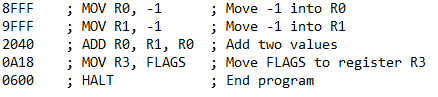
\includegraphics[scale = 1]{NegativeFlags}
		\caption{Testing Latched Flags}
		\label{fig:NegativeFlags}
	\end{figure}
	\bigskip
	The assembly code is below\\
	\begin{tcolorbox}[colback = bg, boxrule = 0pt]
		v2.0 raw\\
		8FFF 9FFF 2040 0A18 0600 \\
	\end{tcolorbox}
	\newpage

	\section{Memory}
	
	\subsection{Question 8.8}
	\begin{tcolorbox}[colback = bg, boxrule = 0pt]
		 A cache has the following parameters: $b$, block size given in numbers of words; $S$, number of sets; $N$, number of ways; and $A$, number of address bits\\

		(a) In terms of the parameters described, what is the cache capacity, $C$?\\
		(b) In terms of the parameters described, what is the total number of bits required to store the tags?\\
		(c) What are $S$ and $N$ for a fully associative cache of capacity C words with block size $b$?\\
		(d) What is $S$ for a direct mapped cache of size $C$ words and block size b?
	\end{tcolorbox}
	\bigskip
	
	(a) The cache capacity is defined as the number of bits that the cache is able to hold. As $S$ tells us how many sets per way, we can define it as 
	\begin{equation}
		S = \frac{B}{N}
	\end{equation}
	Where $B$ is the number of blocks in the cache. We need to solve for $B$, which gives us
	\begin{equation}
		B= SN
	\end{equation}
	As $b$ gives us the block size given in number of words, we get that our cache has a capacity of 
	\begin{equation}
		C = SNb
	\end{equation}
	Our book defines a word as 4 bytes (for a 32 bit ARM CPU) so in terms of bytes, our answer is
	\begin{equation}
		C = 4SNb
	\end{equation}
	\hrule
	\bigskip
	(b) The tag for a cache allows us to check for a hit. By default, if you $S$ sets, then you need 
	\begin{equation}
		SetBits = log_2(S)
	\end{equation}
	We also need to use some bits to determine the number of bits needed for the byte offset, which in our case is simply
	\begin{equation}
		OffsetBits = log_2(b)
	\end{equation}
	This determines the number of offset bits needed. However, Assuming we have $A$ address bits, the number of bits needed for the tag is given by
	\begin{equation}
		TagBits = A - (log_2(S) - log_2(b))
	\end{equation}
	\hrule
	\bigskip
	
	(c) For a full associative cache, all cache blocs are in one set. This means that 
	\begin{equation}
		S = 1
	\end{equation}
	The number of ways, or associativity, of a cache, is the number of blocks in a set. To find the number of blocks, we recognize that the capacity of the cache over the block size in words $b$ gives us the bits per block. In our case, this leads to the equation
	\begin{equation}
		Blocks = \frac{C}{b}
	\end{equation}
	As we have only 1 set in a fully associative cache, the final answer for the number of ways is simply
	\begin{equation}
		N = 1 * (Blocks) = Blocks = \frac{C}{b}
	\end{equation}
	\hrule
	\bigskip
	
	(d) A direct mapped cache is defined as having one block per set. Again, the number of blocks in a cache can be defined as 
	\begin{equation}
		Blocks = \frac{C}{b}
	\end{equation}
	And as each block is its own set, we get
	\begin{equation}
		Sets = Blocks = \frac{C}{b}
	\end{equation}
	
	\subsection{Question 8.10}
	\begin{tcolorbox}[colback = bg, boxrule = 0pt]
		 Repeat Exercise 8.9 for the following repeating sequence of lw addresses (given in hexadecimal) and cache configurations. The cache capacity is still 16 words.
	\end{tcolorbox}
	\begin{figure}[h]
		\centering
		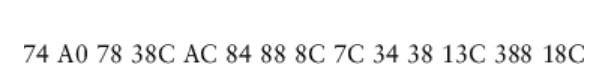
\includegraphics[scale=0.8]{Exercise8.10}
	\end{figure}
	\begin{tcolorbox}[colback = bg, boxrule = 0pt]
		(a) direct mapped cache, b = 1 word\\
		(b) fully associative cache, b = 2 words\\
		(c) two-way set associative cache, b = 2 words\\
		(d) direct mapped cache, b = 4 words
	\end{tcolorbox}
	
	(a) For a direct mapped cache with a block size of 1 word, we will have the two lower bits for the offset and the next 4 for the set, as each block is in its own set. This will give us the following cache memory model
	\newpage
	\begin{table}
		\begin{center}
			\begin{tabular}{c | c}
				Set & Value\\
				\hline\hline
				0 & EMPTY\\
				1 & 84 \\
				2 & 88 388\\
				3 & 38C 8C 18C\\
				4-7 & EMPTY\\
				8 & A0\\
				9 & EMPTY\\
				10 & EMPTY\\
				11 & AC\\
				12 & EMPTY\\
				13 & 74 34\\
				14 & 78 38\\
				15 & 7C 13C\\ 
				\hline
			\end{tabular}
		\end{center}
	\end{table} 
	
	
	As our block size is 1 word, and only 3 hits occur (the values don't change). As such, our miss rate is $1 - \frac{3}{14} = \frac{11}{14}$
	\bigskip
	\hrule
	
	(b) For a fully associative cache with block size 2, each block is in the same set. As such, we expect to have 8 ways. This gives us the cache memory model listed below. We notice that there were only two hits, and as such, that means that our miss rate was $\frac{12}{14}$.
	
	\begin{table}[h]
		\begin{center}
			\begin{tabular}{c | c}
				Set & Value\\
				\hline\hline
				0 & [74, 78]\\
				\hline
				1 & [A0, A4] [13C, 140]\\
				\hline
				2 & [38C, 390] [388, 38C]\\
				\hline
				3 & [AC B0] [18C, 190]\\
				\hline
				4 & [84, 88]\\
				\hline
				5 & [8C, 90]\\
				\hline
				6 & [7C, 80]\\
				\hline
				7 & [34, 38]\\
				\hline
			\end{tabular}
		\end{center}
	\end{table} 

	\hrule
	(c) Using a two way set associative cache with a block size of two words will give us that the total number of sets will be 4. This can be derived by realizing that if we 2 words in each block, and each set maps to one of two ways, we have 4 words per set (evenly split between two ways). As a result, for a 16 bit cache, we will expect that we have $\frac{16}{4} = 4$ sets. So, 2 bits will be used for set after the two bits for the offset. Using this cache model on the addresses given gives us the model below.
	 \newpage
	\begin{table}[h]
		\begin{center}
			\begin{tabular}{c | c}
				Set & Value\\
				\hline\hline
				0 & [A0, A4]\\
				\hline
				1 & [74, 78] [84, 88] [34 38]\\
				\hline
				2 & [389, 390]\\
				\hline
				3 & [38C, 390] [AC, B0] [8C, 90] [7C, 80] [13C, 140] [18C, 190]\\
				\hline
			\end{tabular}
		\end{center}
	\end{table}
	
	From our cache structure, we can see that our miss rate, with the addresses is $\frac{6}{14}$.
	\hrule
	
	(d) For a direct mapped cache with 4 words, we get the a cache with 4 sets, each one holding a block. As such, we have 2 bits after the 2 offset bits for the sets. This gives us the cache model below
	
	\begin{table}[h]
		\begin{center}
			\begin{tabular}{c | c}
				Set & Value\\
				\hline\hline
				0 & [A0, AC]\\
				\hline
				1 & [84, 90] [34, 40] [388 394]\\
				\hline
				2 & [74, 80]\\
				\hline
				3 & [38C, 398] [13C, 148] [18C, 198]\\
				\hline
			\end{tabular}
		\end{center}
	\end{table}
	
	Our miss rate is thus $\frac{7}{14}$ as our hit rate is 50\%.
	
	\subsection{Question 8.14}
	\begin{tcolorbox}[colback = bg, boxrule = 0pt]
		You've joined a hot new Internet startup to build wrist watches with a built-in pager and Web browser. It uses an embedded processor with a multilevel cache scheme depicted in the figure below. The processor includes a small on-chip cache in addition to a large off-chip second-level cache.
	\end{tcolorbox}
	\begin{figure}[h]
		\centering
		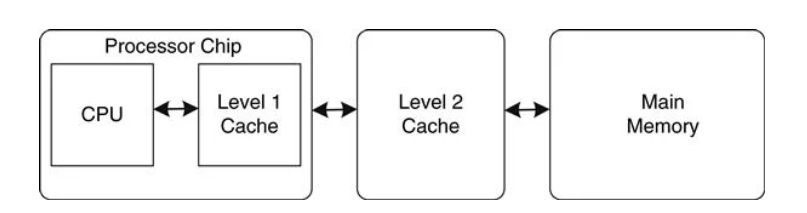
\includegraphics[scale = 1]{System8.14}
		\label{fig:System8.14}
	\end{figure}
	\begin{tcolorbox}[colback = bg, boxrule = 0pt]
		Assume that the processor uses 32-bit physical addresses but accesses data only on word boundaries. The caches have the characteristics given in Table 8.5. The DRAM has an access time of $t_m$ and a size of 512 MB.\\
		
		(a) For a given word in memory, what is the total number of locations in which it might be found in the on-chip cache and in the second-level cache?\\
		(b) What is the size, in bits, of each tag for the on-chip cache and the second-level cache?\\
		(c) Give an expression for the average memory read access time. The caches are accessed in sequence.\\
		(d) Measurements show that, for a particular problem of interest, the on-chip cache hit rate is 85\% and the second-level cache hit rate is 90\%. However, when the on-chip cache is disabled, the second-level cache hit rate shoots up to 98.5\%. Give a brief explanation of this behavior.
	\end{tcolorbox}
	
	\begin{figure}[h]
		\centering
		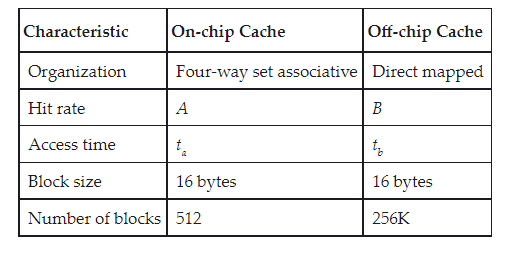
\includegraphics[scale = 1]{Table8.14}
		\label{fig:Table8.14}
	\end{figure}
	
	(a) The total number of locations data can be stored in the cache is simply the block size in the cache multiplied by the number of blocks. As such, this gives us the equation
	\begin{equation}
		OnChip = 512 * 16 = 8192
	\end{equation}
	for the on-chip cache, and 
	\begin{equation}
		OffChip = 16 * 256K = 4096K 
	\end{equation}
	 for the off-chip cache.
	 \bigskip
	 \hrule
	 
	 (b) The on-chip cache is a 4-way set associative cache, meaning that each set has 4 (or blocks). Given that we have 512 blocks on this cache chip, we have a total of
	 \begin{equation}
	 	\frac{512}{4} = 128
	 \end{equation}
 	 sets on the cache, which require a total of 7 bits to represent. We also need 4 bits for the byte offset, as $2^4 = 16$ and a word is 16 bytes. As such, the tag has a total of 
 	 \begin{equation}
 	 	Tag = 32 - (7+4) = 21
 	 \end{equation} 
  	bits for the on-chip cache. As for the off-chip cache, we have a direct mapped cache with 256K blocks, and so have just as many sets. To represent this number, we need 18 bits, as $log_2(262144) = 18$. We also need another 4 bits for the byte offset. This tells us that the tag bits can be described as
  	\begin{equation}
  		TagOffChip = 32-(18+4) = 10
  	\end{equation}
  	bits for the off-chip cache.
  	\hrule
  	
  	(c) The expression for the AMAT of our two three level memory system is shown below
  	\begin{equation}
  		AMAT = t_a + (1-A)(t_b + (1-B)t_m)
  	\end{equation}
  	\hrule
  	
  	(d) The reason for why the off-chip cache system would see an increase in hit rate due to disabling the on-chip cache has to do with the fact that the on-chip cache will mostly hold data that is accessed regularly or being currently operated on - that is, data with a lot of temporal and spatial locality. On the other hand, the off-chip cache will pull data that is accessed occasionally, but not as regularly as the on-chip cache (memory contains data that is rarely accessed). This means that, in general, data that is regularly accessed will count as a hit for the first level cache only, not the second level cache. 
  	
  	However, when you have disabled the on-chip cache, your off-chip cache now contains data that is both regularly accessed and occasionally accessed. This means that you can now expect a hit rate increase for your off-chip cache, which makes the hit rate higher on the off-chip cache. This explains the reasoning for the observation made in this problem.
\end{document}